\documentclass[a4paper,10pt,print]{article}
\usepackage{mathrsfs}
\usepackage{fancyhdr}
\pagestyle{fancy}
\usepackage{verbatim}
\usepackage{graphicx}
\usepackage{bbding}
\usepackage{booktabs}
\usepackage{multirow}
\usepackage{tabularx}
\usepackage{amsmath,amssymb}

\title{\textbf{The inflation of a rubber balloon}}
\author{
%Dingwen Wang\\
%Department of Astronautical Science and Engineering,\\
%School of Aerospace and Materials Engineering,\\
%National University of Defense Technology, Changsha, PR China\\
%wangdingwen0618@gmail.com
%\and Puyun Gao\\
%Department of Astronautical Science and Engineering,\\
%School of Aerospace and Materials Engineering,\\
%National University of Defense Technology, Changsha, PR China
}
\date{}
\begin{document}

\maketitle

\begin{abstract}
The inflation of balloon is realized by the pressure jump across the  membrane.
Here we examine two methods: adding gas and heating up.
In this paper, we give a general and simplified approach to derive the balloon's pressure--radius characteristic.
The result here is in good agreement with other papers.
The formulations relate the inner gas's thermodynamic state to the deformation of balloon are also derived.
Since rubber is incompressible material and its modulus of elasticity is an function of temperature, the behavior of the balloon seems abnormal.
An example illustrates the influence of temperature on the deformation of rubber balloon.
\\
\emph{Key words}: Rubber balloons, Hooke's law, finite deformation, stability, Mooney--Rivlin model
\end{abstract}

\graphicspath{{Figures/}}
\section{Introduction}
The inflation of a rubber balloon refers to the problem of large deformation\cite{Rivlin,Green Zerna,Green Shield,Atkins Rivlin}.
To analyse or simulate the process, it is important to choose the material law\cite{Atkins Rivlin,Muller Struchtrup}.
Mooney--Rivlin model is always used. And results from this model are compared with the experimental datas\cite{Atkins Rivlin}.
M\"{u}ller and Struchtrup simulate the process of inflating a single balloon by mouth\cite{Muller Struchtrup}.

In this paper, we study the process from another aspect.
To inflate a balloon, we need some gas to fill it.
Then the thermodynamic state of the inner gas is coupled with the strain or the stress of balloon.
Usually, we inflate the balloon by two methods: adding more gas into the balloon or heating up the gas to expand the balloon, see Figure \ref{myfigure1} and Figure \ref{myfigure2}.
The two methods will be studied in this paper.
And we will show how the thermodynamic state of gas and the environmental temperature influence the inflation of balloon.
For simplicity, we always assume the atmosphere pressure to be $0\text{ Pa}$.
\begin{figure}[!hbt]
  \centering
  % Requires \usepackage{graphicx}
  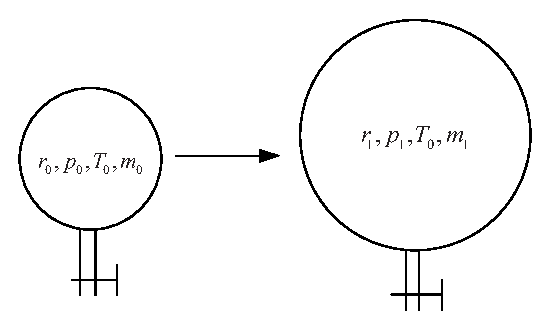
\includegraphics[scale=0.8]{inflating1.eps}\\
  \caption{Add gas}\label{myfigure1}
\end{figure}
\begin{figure}[!hbt]
  \centering
  % Requires \usepackage{graphicx}
  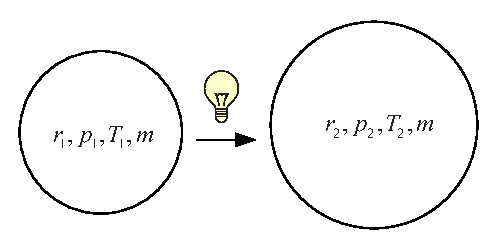
\includegraphics[width=8cm]{inflating2.eps}\\
  \caption{Heat up}\label{myfigure2}
\end{figure}

\section{Inflating by adding gas}

Consider a spherical rubber balloon inside which the mass of the gas is $m_0$ and the inner pressure is $p_0$.
Assuming the gas as an ideal gas, that means it obeys the ideal gas state law.
The radius of the balloon is $r_0$, and the thickness of the balloon membrane is $t_0(t_0 \ll r_0)$.
This is called the \emph{initial configuration}.

To get the $p-r$ characteristic, which dictates the dependence of the pressure difference across the membrane of the spherical balloon on the radius $r$, we first study the first method which indicates adding more gas.

The balloon is inflated, for example, by mouth or some inflation apparatus.
This is an isothermal process which means the temperature will not change during inflating.
The pressure is increased to $p_f$, and the mass of gas is $m_f$.
The balloon assumes a spherical shape with final radius $r_f=\beta r_0$, where $\beta >1$.
This can be called the \emph{final configuration}.
Since this is a thin membrane balloon, both the initial membrane thickness $t_0$ and the final one $t_f$ are small($t_0\ll r_0$,$t_f\ll r_f$).

In order to get the pressure-radius characteristic, it is necessary to express the membrane stress $\sigma_0$ and $\sigma_f$ in terms of geometry and internal pressure.
Since we have assumed that both configurations remain spherical, we will know the relationship between the membrane stress $\sigma$ and the inner pressure $p$:

\begin{equation}\label{stressandpressure}
  \sigma=\frac{p r}{2 t}
\end{equation}



Here we have two approaches to get the $p-r$ characteristic which will be shown below.
\subsection{Euler Strain}
This approach can be seen in \cite{internet}.In this literature, it uses the Eulerian strain measure.
The average circumferential extensional strain is
\begin{equation}\label{eulerstrain}
  \epsilon_f^E=\frac{2 \pi (r_f-r_0)}{2 \pi r_f}=\frac{\beta-1}{\beta}
\end{equation}
The strains are assumed to be zero in the initial configuration.

 Since the balloon is assumed to remain spherical and its thickness is very small compared to its radius, then the strains hold at all points of the balloon membrane, and are the same in any direction tangent to the sphere.
 If we choose the sphere normal as local z axis, the membrane is in a plane stress state.
 We assume the rubber obeys the two-dimensional, plane stress generalized Hooke's law with respect to the Eulerian strain measure, with effictive modulus of elasticity $E$ and Poisson's ratio $\nu$.
 Choosing $\epsilon_{xx}=\epsilon_{yy}=\epsilon_f^E$ and $\gamma_{xy}=0$ and accounting for the initial stress $\sigma_0$, we get the membrane stress in the final configuration:
 \begin{equation}\label{stress}
   \sigma_{xx}=\sigma_{yy}=\sigma_f=\sigma_0+\frac{E}{1-\nu^2}(\epsilon_f^E+\nu \epsilon_f^E)=\sigma_0+\frac{E}{1-\nu} \epsilon_f^E=\sigma_0+\frac{E}{1-\nu} \frac{\beta-1}{\beta}
 \end{equation}
 The inplane shear stress $\tau$ vanishes in all directions.

 From (\ref{stressandpressure}) we can know:
 \begin{equation}\label{inandfnstress}
    \sigma_0=\frac{p_0 r_0}{2 t_0},\qquad  \sigma_f=\frac{p_f r_f}{2 t_f}=\frac{p_f\beta r_0}{2 t_f}
 \end{equation}
 All quantities in the above expressions can be known if given the initial data, except $t_f$.
 A kinematic analysis shows that \cite{internet}:
 \begin{equation}\label{thickness}
   t_f=[1+2\nu(\frac{1}{\beta^2}-1)]t_0
 \end{equation}
Substitute (\ref{thickness}) into (\ref{inandfnstress}.2), equate this to (\ref{stress}) and solve for $p$. Then the result is
 \begin{equation}\label{pressure1}
   p=\frac{2 E t_0 (\beta-1)(2 \nu+\beta^2(1-2\nu))+ r_0 p_0 \beta(1-\nu)(4\nu+\beta^2(2-\beta-4\nu))}{ r_0 \beta^4(1-\nu)}
 \end{equation}
\subsection{Membrane Energy}
We can get the $p-\beta$ characteristic through a more general method---the energy method.
The work done by the gas pressure must be equal to the increment of the membrane strain energy
\begin{equation}\label{Energy}
  W=\Delta \mathscr{U}
\end{equation}
Consider a infinitesimal inflating process, then (\ref{Energy}) becomes to
\begin{equation}\label{energy}
  p dV  = d V_m \mathscr{E}(\sigma)
\end{equation}
$V=\frac{4}{3}\pi r^3$ is the volume of the gas inside the balloon.
$V_m$ is the volume of the thin--wall spherical balloon membrane.
The membrane strain energy density $\mathscr{E}$  is a function of the membrane strain or stress $\sigma$.
Expanding (\ref{energy}) yields to
\begin{equation}\label{energy1}
  4 \pi r^2 p dr=d V_m \mathscr{E}(\sigma)
\end{equation}
Since $r=\beta r_0$, we can rewrite (\ref{energy1}) as
\begin{equation}\label{energy2}
  4 \pi r_0^3 p \beta ^2d\beta=d V_m \mathscr{E}(\sigma)
\end{equation}
If given  the membrane strain energy density $\mathscr{E} $ in terms of the membrane stress $\sigma$, in other words the constitutive model, we will relate the membrane stress $\sigma$ to the balloon radius ratio $\beta$. Finally we will know the $p-\beta$ characteristic using formula (\ref{stressandpressure}).

The key point is how we define the membrane energy density $\mathscr{E}$ or the constitutive law.
Rubber is highly nonlinear or hyperelastic material.
There are a lot of hyperelasticity models to describe hyperelastic material behavior, such as the Mooney--Rivlin, Ogden, and Arruda--Boyce models\cite{hyperelastic}.
But for simplicity and in order to compare the two methods, we choose the Hooke's model as the constitutive equation here.
That means the material constants are modulus $E$ and Poisson's ratio $\nu$.

From equation (\ref{thickness}), we can express $V_m$ as
\begin{equation}\label{volumem}
  V_m=4 \pi r^2 t=4 \pi r_0^2 \beta^2(1+2 \nu (\frac{1}{\beta^2}-1))t_0
\end{equation}
And using (\ref{stressandpressure}) we derive:
\begin{equation}\label{pressureandstressfinal}
  p=\frac{2\sigma t}{r}=\frac{2\sigma(1+2\nu(\frac{1}{\beta^2}-1)) t_0}{r_0 \beta}
\end{equation}
Substituting (\ref{volumem}) and (\ref{pressureandstressfinal}) into (\ref{energy2}) yields
%\begin{eqnarray}
% \nonumber to remove numbering (before each equation)
%   4 \pi r_0^3 \beta^2 \frac{2\sigma(1+2\nu(\frac{1}{\beta^2}-1)) t_0}{r_0 \beta} d\beta &=& d 4 \pi r_0^2 \beta^2(1+2 \nu (\frac{1}{\beta^2}-1))t_0 \mathscr{E}(\sigma) \\
 % \beta^2 \frac{2\sigma(1+2\nu(\frac{1}{\beta^2}-1))d\beta&=& d \beta^2(1+2\nu(\frac{1}{\beta^2}-1))\mathscr{E}(\sigma)
%end{eqnarray}

\begin{equation}\label{energy3}
   4 \pi r_0^3 \beta^2 \frac{2\sigma(1+2\nu(\frac{1}{\beta^2}-1)) t_0}{r_0 \beta} d\beta = d 4 \pi r_0^2 \beta^2(1+2 \nu (\frac{1}{\beta^2}-1))t_0 \mathscr{E}(\sigma)\end{equation}
Simplifying (\ref{energy3}), we get
\begin{equation}\label{energy4}
     \frac{2\sigma(\beta^2+2\nu(1-\beta^2)) }{ \beta} d\beta = d(\beta^2+2 \nu (1-\beta^2)) \mathscr{E}(\sigma)
\end{equation}
Define
\begin{equation}\label{f_function}
  f(\beta):=\beta^2+2\nu(1-\beta^2)
\end{equation}
Then (\ref{energy4}) can simply expressed as
\begin{equation}\label{energy5}
  \frac{2\sigma f(\beta)}{\beta}d \beta=df(\beta) \mathscr{E}(\sigma)
\end{equation}

We already know the stresses are the same at all points of the balloon's membrane and also the same in any direction tangent to the sphere.
If we choose the sphere normal as local $z$ axis, the wall is in a plane stress state.
Then the membrane energy density is
\begin{equation}\label{energydensity}
  \mathscr{E}=\frac{(1-\nu)\sigma^2}{E}
\end{equation}
Substituting (\ref{energydensity}) to (\ref{energy5}) yields
\begin{equation}\label{energy6}
  f(\beta)\frac{2(1-\nu)}{E}\sigma d \sigma=(\frac{2 \sigma f(\beta)}{\beta}-\frac{f'(\beta)(1-\nu)\sigma^2}{E})d \beta
\end{equation}

This is a first order differential equation about $\sigma$ in term of $\beta$. With the initial value $\sigma(\beta=1)=0$, we can get the analytical solution.

Rubber is always considered as incompressible, it suggests that Possion's ratio $\nu=\frac{1}{2}$, then the solution of (\ref{energy6}) provided by \emph{Mathematica} is
\begin{equation}\label{solution}
  \sigma(\beta)=2E \rm{ln} (\beta)
\end{equation}

With (\ref{inandfnstress}) and (\ref{thickness}), we have the final pressure--radius characteristic from (\ref{solution})
\begin{equation}\label{final}
  p(\beta)=\frac{4 E t_0 \rm{ln} \beta}{\beta^3 r_0}
\end{equation}

Now let's consider from another aspect.
From equation(\ref{solution}), the relation between $\sigma$ and $r$ is
\begin{equation}\label{relation}
  \sigma_2-\sigma_1=2E \rm{ln}(\frac{r_2}{r_1})
\end{equation}

Then
\begin{equation}\label{relation1}
  \frac{p_2 r_2}{2 h_2}- \frac{p_1 r_1}{2 h_1}=2E \rm{ln}(\frac{r_2}{r_1})
\end{equation}

Since rubber is incompressible($\nu=\frac{1}{2})$, the volume the membrane is constant.
\begin{equation}\label{relation2}
  \frac{p_2 r_2}{2 h_2}- \frac{p_1 r_1}{2 h_1}=\frac{p_2 r_2^3}{2 h_2 r_2^2}- \frac{p_1 r_1^3 }{2 h_1 r_1^2}=\frac{2\pi}{V_m}(p_2 r_2^3-p_1 r_1^3)=2E \rm{ln}(\frac{r_2}{r_1})
\end{equation}

From the ideal gas state law, we have
    \begin{equation}\label{idealgas}
     \left\{ {\begin{array}{*{20}{c}}
    {p_1 \frac{4\pi}{3}r_1^3=m_1 R_M T_1}\\
    {p_2 \frac{4\pi}{3}r_2^3=m_2 R_M T_2}\\
    \end{array}} \right.
    \end{equation}
$R_M$ is gas constant, $m$ is the mass of gas.
This is an isothermal process, so $T_1=T_2=T_0$. Then (\ref{relation2}) becomes
\begin{equation}\label{relation3}
  \frac{3}{2 V_m} R_M T_0(m_2-m_1)=2E \text{ln}\frac{r_2}{r_1}
\end{equation}

Finally we get
\begin{equation}\label{relation4}
  r_2=r_1 \text{exp}\Big(\frac{3 R_M T_0}{4E V_m}(m_2-m_1)\Big)
\end{equation}
The mass of gas to inflate the balloon can be calculated from (\ref{relation4}).

\subsection{Comparison between different models}
Now we have the pressure--radius characteristics from two approaches.
They are not exactly the same.
Assuming $p_0=0$ and $\sigma_0=0$, we get
         \begin{equation}\label{comparison}
         \left\{ {\begin{array}{*{20}{l}}
         {p(\beta)=\frac{4 E t_0 (\beta-1)}{ \beta^4 r_0 } \qquad (\text{euler-strain})}\\
         {p(\beta)=\frac{4 E t_0 \rm{ln} \beta}{\beta^3 r_0} \qquad (\text{hooke membrane energy})}\\
         \end{array}} \right.
         \end{equation}

The curves given by (\ref{comparison}) are plotted in Figure \ref{myfigure3}.
The two curves generally have the same trend but the curve of membrane energy approach is higher than the curve of Euler-strain approach especially when $\beta$ is large.
This is because the strain in membrane energy approach include the finite deformation which is more accurate than Euler-strain approach.
\begin{figure}[!htb]
  \centering
  % Requires \usepackage{graphicx}
  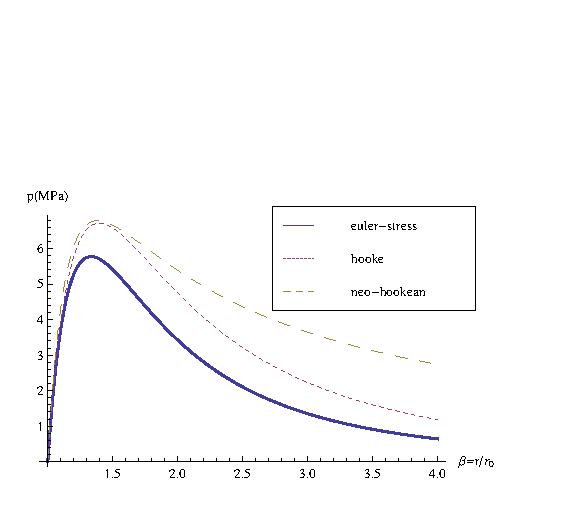
\includegraphics[width=10cm]{figure.eps}\\
  \caption{Comparison of inflating pressure(in MPa) radius characteristics for a balloon with $E=1900\text{MPa}$, $r_0=25\text{mm}$, $p_0=0\text{MPa}$, $t_0=0.18\text{mm}$, $1\leq \beta \leq 4$, Poisson's ratio $\nu=\frac{1}{2}$, and $C_1=380\text{Mpa}$.}\label{myfigure3}
\end{figure}

The membrane strain energy appoach is also effective when we choose a hyperelastic model, say neo-Hookean model.
For an incompressible rubber, we will get
\begin{equation}\label{moonyrivlin}
  p(\beta)=\frac{4 t_0}{r_0 \beta}C_1(1-\frac{1}{\beta^6})
\end{equation}
from (\ref{energy}). The membrane strain energy density is $\mathscr{E}=C_1(I_1-3) $. $I_1=2 \beta^2+1/ \beta^4$ and $C_1$ is a constant.
This is in good agreement with the result in \cite{Green Shield}.

It is also interesting that the pressure--radius characteristic is not monotonic.
This is important when two balloon of different radii are interconnected, see\cite{Atkins Rivlin,Muller Struchtrup,Dreyer Muller}.

The value of $\beta$ for which $p$ has a stationary value can be obtained analytically by solving the equation $dp/d\beta=0$.
For the Hooke membrane energy density model, it happens when $\beta=e^{1/3}\approx 1.39561$.
This is very close to the neo--Hookean model which suggests $\beta=\sqrt[6]{7}\approx 1.38309$.
So it is reasonable to choose Hooke's model here. All the three models are shown and compared in Figure \ref{myfigure3}.
\section{Inflating by heating}
We can also inflate a rubber balloon by heating up the balloon.
Then the gas inside will dilate to expand the balloon.
But another problem arises.
Since the rubber modulus of elasticity can increase when temperature grow, the balloon may deflate even the inner pressure increase which we will see below.
For simplicity, assume
\begin{equation}\label{modulus}
  E(T)=E_0+\alpha (T-T_0)
\end{equation}
in some temperature range, $\alpha$ is a constant.

The balloon rushes into a hot environment, which means the environmental temperature is higher than the balloon and the gas inside.
The thermal conductivity is much larger in solid than in gas; so we assume the rubber will reach the final temperature immediately and the gas will remain the initial temperature at the same time.
We divide the inflating process into two steps.
Step I: for the rubber reaches the final temperature instantaneously the balloon will deflate due to the rubber's modulus of elasticity increases while the inner gas remains the same temperature.
This step will be completed very soon.
Step II: then the balloon will inflate because the gas dilates according to temperature rising.


We will know at the end of Step I, the radius of the balloon changes from $ r_1=r_0exp(\frac{3 R_M T_0}{4E(T_0) V_m}m)$ to
\begin{equation}\label{relation5}
  r_1'=r_0\text{exp}\Big(\frac{3 R_M T_0}{4E(T) V_m}m\Big)
\end{equation}
$m$ is the mass of gas inside the balloon. To derive (\ref{relation5}),we need only change $E(T_0)$ to $E(T)$ and consider (\ref{relation}) and (\ref{idealgas}).
In this step temperature of the inner gas remains $T_0$ while the membrane's temperature rises to $T$.

Remember we have assumed the atmosphere pressure is $0 \text{ Pa}$, then at the end of Step II we have
\begin{equation}\label{relation6}
  \frac{3}{2 V_m} R_M m(T_2-T_1)=2E(T) \text{ln}\frac{r_2}{r_1'}
\end{equation}
it means
\begin{equation}\label{relation7}
  r_2=r_1' \text{exp}\Big(\frac{3 R_M m}{4E(T) V_m}(T-T_0)\Big)
\end{equation}


Substituting (\ref{relation5}) to (\ref{relation7}), we finally get
\begin{equation}\label{relation8}
  r_2=r_1' \text{exp}\Big(\frac{3 R_M m}{4E(T) V_m}(T-T_0)\Big)=r_0 \text{exp}\Big(\frac{3 R_M m}{4E(T) V_m}T\Big)
\end{equation}
This equation shows the radius of balloon changes from $r_1$ to $r_2$ when temperature rises from $T_0$ to $T$ .
\section{Example}

Now let's consider an example which indicates the balloon's abnormal behavior when temperature changes.

A balloon is inflated by mouth, and the environmental temperature is $300\text{ K}$.
The balloon expands until the radius ratio reach $\beta=1.2$.
Then we move the balloon to a new environment whose temperature is $310\text{ K}$.
The questions are what is the mass of gas inside the balloon and what is the final radius ratio.

We assume the modulus of elasticity changes like this: $E(T)=1900+10(T-300) \text{ Mpa}$.
The air's $R_M=286.91 \text{ J}\cdot \text{K}^{-1} \cdot \text{kg}^{-1}$.
The balloon's initial configuration: $r_0=25\text{ mm}$, $p_0=0\text{ MPa}$, $t_0=0.18\text{ mm}$, and the atmosphere pressure is set to zero for simplicity.

The mass of the air inside the balloon can be calculated from (\ref{relation4}): $m=7.58623\times10^{-3}\text{ kg}$.
The inner pressure is $5.77352\text{ MPa}$ from (\ref{final}).

After the balloon moves to the environment of temperature $310\text{ K}$, the final radius ratio is $\beta'=1.196$ from (\ref{relation8}).
The inner pressure becomes to $6.02615\text{ MPa}$.

It is interesting here that the balloon deflates($\beta= 1.2\longrightarrow1.196$) though the inner pressure of balloon increases.
More of the rubber's abnormal behavior due to the change of temperature can be seen in \cite{Shedd Ingersol}.

\section{Conclusion}
Two methods to inflate a rubber balloon have been studied.
The balloon's pressure--radius characteristic is derived from different approaches.
The result shown here suggests that the $p-\beta$ characteristics derived from Hooke model and Moony--Rivlin model are very close when $\beta$ is not large ($1<\beta<1.5$).
The relation between the thermodynamic state of inner gas and the membrane's stress are also displayed.
Temperature plays a peculiar role when we inflate balloon by heating up.
Example given here shows the balloon may deflate when temperature rises.
This is because temperature influence rubber's modulus of elasticity.
Inversely, the balloon may inflate when temperature descends.
This is important when a balloon rises from ground to high space where temperature is very low.



\begin{thebibliography}{99}
\setlength{\parskip}{0pt}  %����֮�����ֱ����
\bibitem{Rivlin}Rivlin R.S.Large Elastic Deformations of Isotropic Materials. II. Some Uniqueness Theorems for Pure, Homogeneous Deformation. Phil. Trans. R. Soc. Lond. A  240, 491-508 (1948).
\bibitem{Green Zerna}Green A.E. and Zerna E. XXVI. Theory of elasticity in general coordinates., Philosophical Magazine Series 7, 41, 315, 313-336 (1950)
\bibitem{Green Shield} Green, A.E. and Shield, R.T. Finite Elastic Deformation of Incompressible Isotropic Bodies. Proc. R. Soc. Lond. A 202, 407-419 (1950).
\bibitem{Atkins Rivlin}Atkins, J.E. and Rivlin, R.S. Large Elastic Deformations of Isotropic Materials. IX. The Deformation of Thin Shells, Phil. Trans. R. Soc. Lond. A 244, 505-531 (1951).
\bibitem{Muller Struchtrup}M\"{u}ller, I. and Struchtrup, H. Inflating a Rubber Balloon. Mathematics and Mechanics of Solids, 7, 569-577 (2002).
\bibitem{internet}{http://www.colorado.edu/engineering/CAS/courses.d/Structures.d/\\ASEN3112.Lect05.d/ASEN3112.Lect05.pdf}
\bibitem{hyperelastic}Boyce M.C., Arruda E.M. Constitutive models of rubber elasticity: a review. Rubber Chemistry and Technology, 73, 504-523 (2000).
\bibitem{Dreyer Muller}Dreyer, W., M\"{u}ller, I. and Strehlow, P. A Study of Equilibria of Interconnected Balloons.  Q. J. Mech. Appl. Mech., 35, 419-440 (1982).
\bibitem{Shedd Ingersol}Shedd J.C. and Ingersol R.L. The Elastic Modulus and Elastic Limit of Rubber and Theri Relation to Change of Temperature. Phys. Rev. (Series I) 19, 107-116 (1904).
\end{thebibliography}


\end{document}
